\documentclass[12pt]{article}
\usepackage{amsmath,amssymb}
\textheight 240mm
\textwidth  170mm
\oddsidemargin  0mm
\evensidemargin 0mm
\topmargin -20mm

\usepackage[utf8]{inputenc}
\usepackage{graphicx}
\usepackage{float}
\usepackage{titling}
\usepackage{geometry}
\usepackage{color}

\geometry{ a4paper,
	left=30mm,
	right=30mm,
	top=20mm,
}

\addtolength{\headheight}{0.2pt}
%\setlength{\droptitle}{-8em}

\title{Music Genre Classification}
\author{Abhijit Suresh, Paria Rezaeinia, Sahana Sadogopan}

\begin{document}
	\maketitle

\section{Introduction}

Music genre classification is the task of classifying the given audio signal into its corresponding categorical description (a.k.a. genre). It has been a very challenging task in the field of music information retrieval (MIR) and widely used for digital music service and internet radio.  \textcolor{red}{Paria}

%_________________________________________________________________
You will properly define the genre classification problem, and
indicate a few references to the literature.
%_________________________________________________________________
explaining the problem, the current and common methods to solve this problem. the way that we approach it, the algorithms that we use and the reason we use these algorithms. a very brief overview of the results. The organization of the paper. : \textcolor{red}{Paria}
\section{Dimensionality Reduction}
%_________________________________________________________________
Describe your dimension reduction technique, and justify why it
is appropriate to use it in this context. You should explain what
performance is expected.
%_________________________________________________________________
I suggest we give some background to dimensionality reduction and also mention the Johnson-Lindestrauss theorem here. : \textcolor{red}{Sahana}
\subsection{mfcc} \textcolor{red}{Sahana}

\subsection{PCA} \textcolor{red}{Sahana}

\subsection{Content based similarity}
Beth and Ariel[1] presents a novel approach to compare songs based on their corresponding audio content. For each song in the dataset, they create a song signature. The song signature is generated based on k-means clustering of spectral features. The algorithm is summarized in figure below.

\begin{figure}[h]
\center
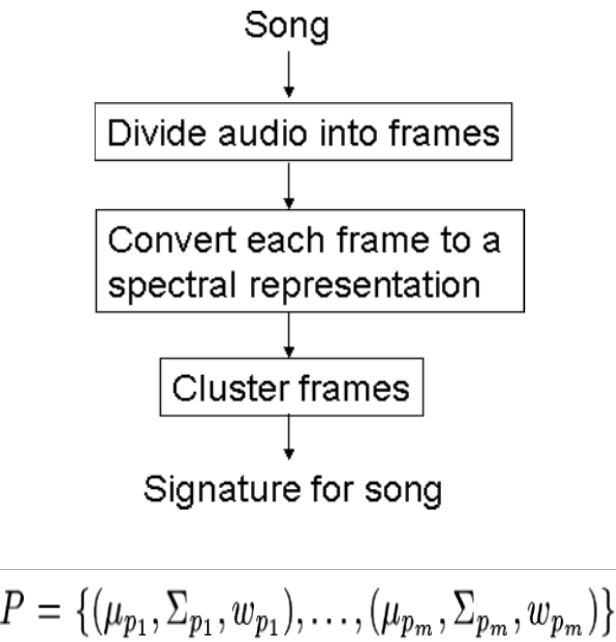
\includegraphics{fig1.png}
\caption{Content based similarity method}
\end{figure}

The first setup is to divide the audio into frames. Then, each frame is converted into its corresponding spectral representation. In order to generate the spectral representation we make use of mfcc algorithm which is explained in the previous sub section. The number of cepstrum coefficients was calculated based on the Johnson-Lindenstrauss lemma.

\subsubsection{Johnson-Lindenstrauss}
The idea behind Johnson-Lindenstrauss lemma
is that points in high-dimensional space can be projected onto low dimensional space while preserving the distance between the points. For a given dataset, the minimum number of dimension required to preserve the distance between the points is given by the formula $$ n > 8 * ln(m) * \epsilon ^ 2 $$ where $\epsion$ is a number between 0 and 1. For this project we have $$ n > 77$$ and hence the number of cepstrum coefficients that we have considered is 79.

\subsubsection{k-Means}
Once each frame is clustered into its corresponding we spectral representation, we cluster the frames using unsupervised k-Means clustering algorithm where the value of k is  fixed to 10. k-Means is a popular clustering algorithm used in data mining. It is often confused with k-nearest neighbour algorithm which makes use of supervised labels during the training phase in order to cluster the points. Given a set of n observations in a d dimensional space, k-Means aims to cluster the n dimension into k sets $S = {S_1,S_2,...S_k}$ where $ k \leq n$. The idea is to find the sum of distance functions of each point in the cluster to the K center. The equation is given by:

\begin{figure}[h]
\center
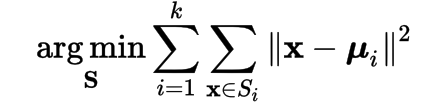
\includegraphics{fig2.png}
\caption{k-Means}
\end{figure}

\subsection{Modified Gaussian Mixture} \textcolor{red}{Paria}

\section{Distance Metrics}
Explain what are the available distance in the space of songs.
Describe your distance and any pre-processing performed before
computing the distance. : \textcolor{red}{Abhijit}
%_________________________________________________________________
\subsection{Minowski distance}\textcolor{red}{Abhijit}
\subsection{Earth Movers distance}\textcolor{red}{Abhijit}
\subsection{Euclidean distance}\textcolor{red}{Paria}
\subsection{Kullback-Leibler distance (KL) distance}\textcolor{red}{Paria}

\section{Statiscal learning}
%_________________________________________________________________
Explain how the training data help find the genre of an unknown
song. This could be as simple as finding the closest song among all
the songs for which you know the genre. Or it could involve more
sophisticated methods. \textcolor{red}{Paria}
%_________________________________________________________________

\subsection{kNN}\textcolor{red}{Paria}

\subsection{Modified-kNN}\textcolor{red}{Paria}

\subsection{Neural Network}\textcolor{red}{Sahana}
\section{Experiments}
%_________________________________________________________________
Describe the experiments, and include the confusion matrix. Discuss
the influence of the various parameters, and describe how the optimal
parameters were chosen. Include the computation time for your method. : \textcolor{red}{Sahana}
%_________________________________________________________________
\section{Discussion}
%_________________________________________________________________
Provide a critique of the approach and discuss any potential
improvement. Discuss the ability of your approach to classify
non-classical into the five remaining genres. \textcolor{red}{Abhijit}
\begin{thebibliography}{9}
	\bibitem{logan}
	Logan, B., & Salomon, A. (2001). A content-based music similarity function. Cambridge Research Labs-Tech Report.
\end{thebibliography}
\end{document}